% This example is meant to be compiled with lualatex or xelatex
% The theme itself also supports pdflatex
\PassOptionsToPackage{unicode}{hyperref}
\documentclass[aspectratio=1610, 9pt, xcolor=dvipsnames]{beamer}
\usepackage{graphicx,caption}
\parskip0pt
% Load packages you need here
\usepackage{polyglossia}
\setmainlanguage{german}

\usepackage{csquotes}

\usepackage{tikz}

\usepackage{subfig}

\usepackage[export]{adjustbox}

\usepackage{amsmath}
\usepackage{amssymb}
\usepackage{mathtools}

\usepackage{hyperref}
\usepackage{bookmark}
\usepackage{graphicx}
\usepackage{wrapfig}

\usepackage{booktabs}

\usepackage{multicol}

\usepackage{relsize}

\usepackage[dvipsnames]{xcolor}

\usepackage{empheq}
\newcommand*\widefbox[1]{\fbox{\hspace{2em}#1\hspace{2em}}}

\makeatletter
\newcommand{\Pause}[1][]{\unless\ifmeasuring@\relax
\pause[#1]%
\fi}
\makeatother

\usepackage[
locale=DE,
separate-uncertainty=true, % Immer Unsicherheit mit ±
per-mode=symbol-or-fraction, % m/s im Text, sonst \frac
% alternativ:
% per-mode=reciprocal, % m s^{-1}
% output-decimal-marker=., % . statt , für Dezimalzahlen
]{siunitx}

% load the theme after all packages

\usetheme[
  showtotalframes, % show total number of frames in the footline
]{tudo}

% Put settings here, like
\unimathsetup{
  math-style=ISO,
  bold-style=ISO,
  nabla=upright,
  partial=upright,
  mathrm=sym,
}

\DeclarePairedDelimiter{\bra}{\langle}{\rvert}
\DeclarePairedDelimiter{\ket}{\lvert}{\rangle}
\DeclarePairedDelimiterX{\braket}[2]{\langle}{\rangle}{
#1 \delimsize| #2
}

%----------------------------------------
%Align Equations to LEFT MARGIN (use \mathleft then \mathcenter)
\makeatletter
\newcommand{\mathleft}{\@fleqntrue\@mathmargin0pt}
\newcommand{\mathcenter}{\@fleqnfalse}
\makeatother
%----------------------------------------

\title{Mn-Verunreinigungen in Graphen: Eine
Tight Binding Modellierung}
\author[Y.~Kind]{Yanick Kind}
\institute[AG Anders]{AG Anders \\  Fakultät Physik}
\date{15. August 2022}
%\titlegraphic{\includegraphics[width=0.7\textwidth]{images/tudo-title-2.jpg}}


\begin{document}

\maketitle

\begin{frame}{Übersicht}
  \begin{columns}
    \column{0.4\linewidth}
    \setlength{\parskip}{4ex}
    \tableofcontents
    \column{0.6\linewidth}
    \vspace*{1cm}
    \centering
    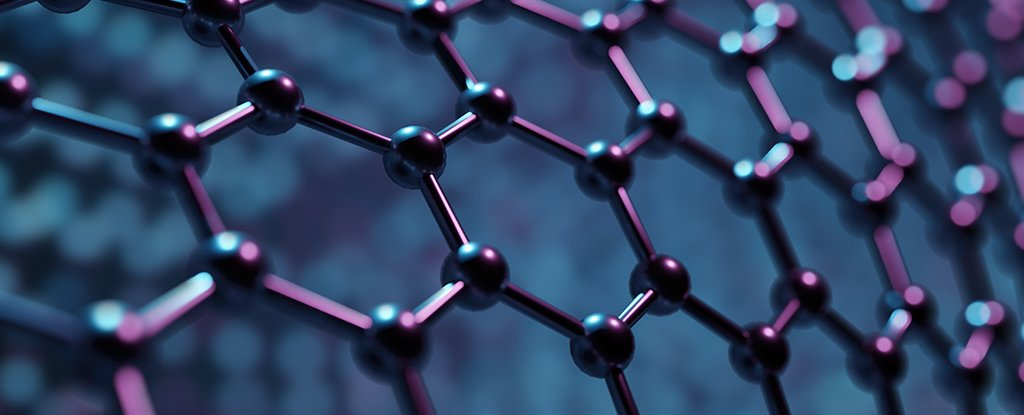
\includegraphics[width = \textwidth]{Plots/rendering.jpg}
    \hspace*{12pt}\hbox{\scriptsize {\footnotesize\itshape \href{https://www.sciencealert.com/graphene}{sciencealert.com/graphene}}}
  \end{columns}
\end{frame}

\section{Einleitung}
\begin{frame}{Motivation}
     $\quad \quad \quad \quad \quad \quad \quad \quad \quad \quad \quad \quad \quad \quad \quad \quad \quad \quad \quad \quad \quad \quad \quad \quad \quad \quad
     \quad \quad \quad \quad \quad \quad \quad \quad \quad \quad \quad \quad$
     Rastertunnelmikroskopie
  %\vspace*{1cm}
  \centering
  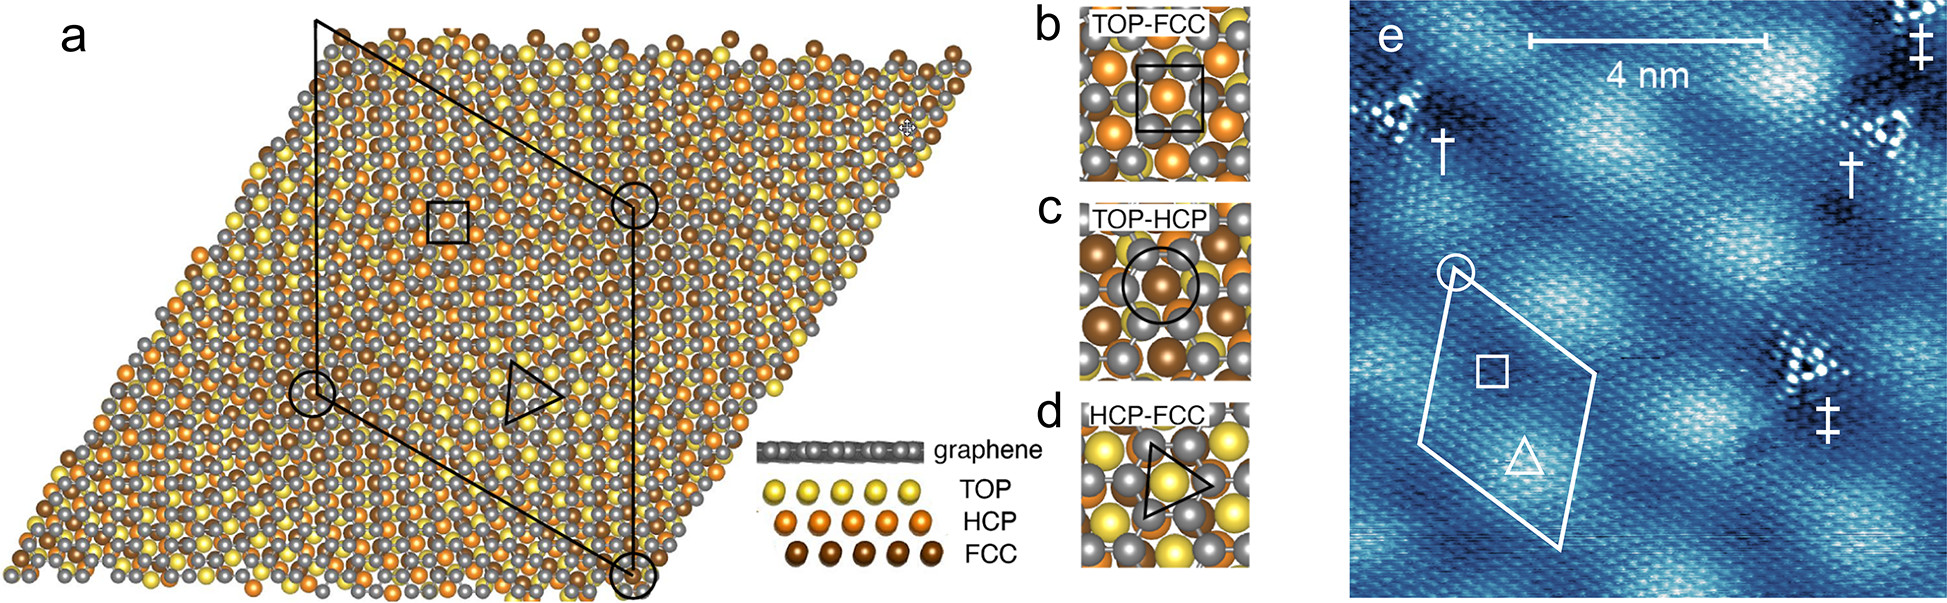
\includegraphics[width = \textwidth]{Plots/images_large_nn1c00139_0002.jpeg}
  \hspace*{12pt}\hbox{\scriptsize {\footnotesize\itshape \href{https://pubs.acs.org/doi/10.1021/acsnano.1c00139}{Pin-Cheng Lin et al., \textit{ACS Nano 15.3 (2021)}}}}
\end{frame}
  \begin{frame}{Motivation}
    \begin{flushleft}
      $\quad \quad \quad \quad \quad$ Rastertunnelmikroskopie
    \end{flushleft}
    \vspace*{-0.27cm}
    \centering
  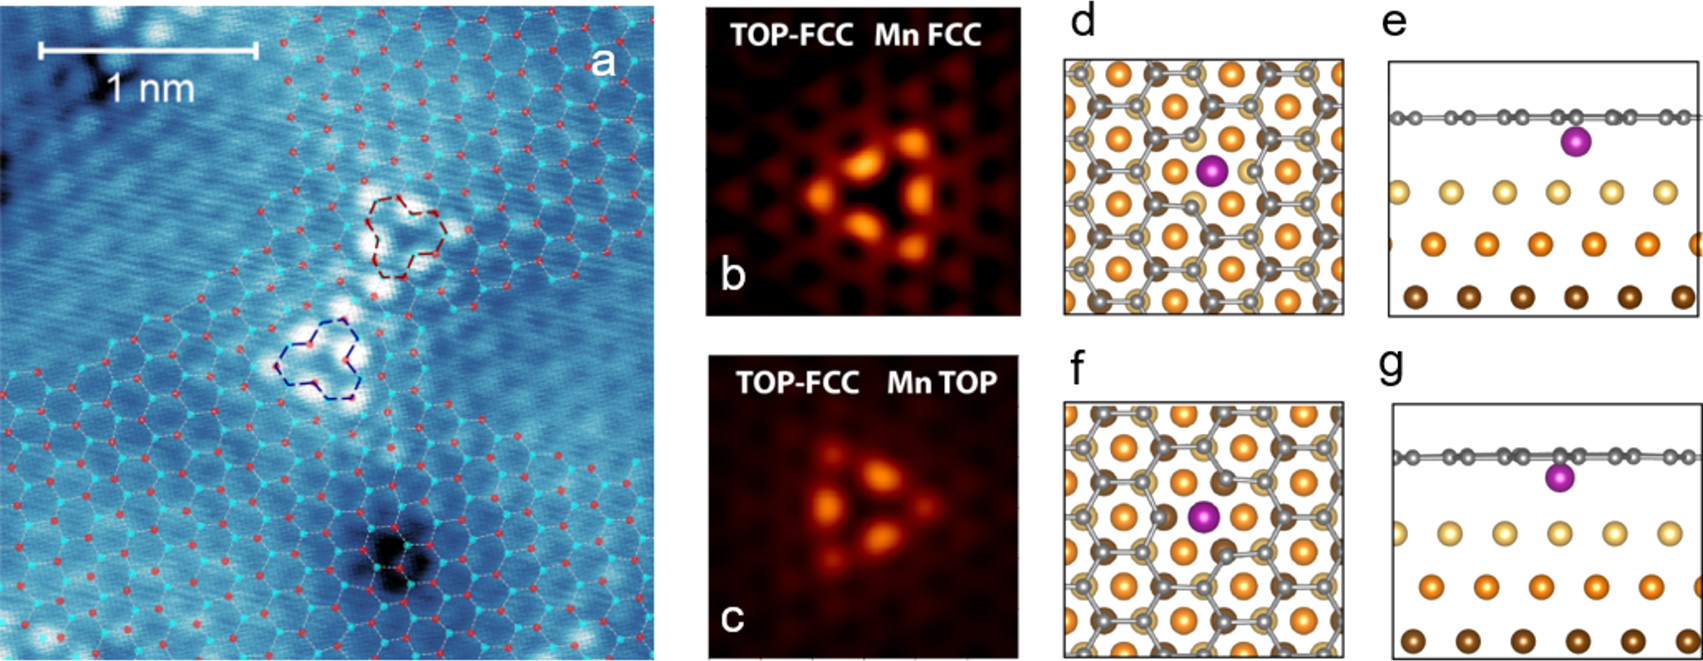
\includegraphics[width = \textwidth]{Plots/images_large_nn1c00139_0003.jpeg}
  \hspace*{12pt}\hbox{\scriptsize {\footnotesize\itshape \href{https://pubs.acs.org/doi/10.1021/acsnano.1c00139}{Pin-Cheng Lin et al., \textit{ACS Nano 15.3 (2021)}}}}
\end{frame}

\begin{frame}{Struktur von Graphen und der Störstelle}
  \begin{columns}
     \column{0.45\linewidth}
        \centering
        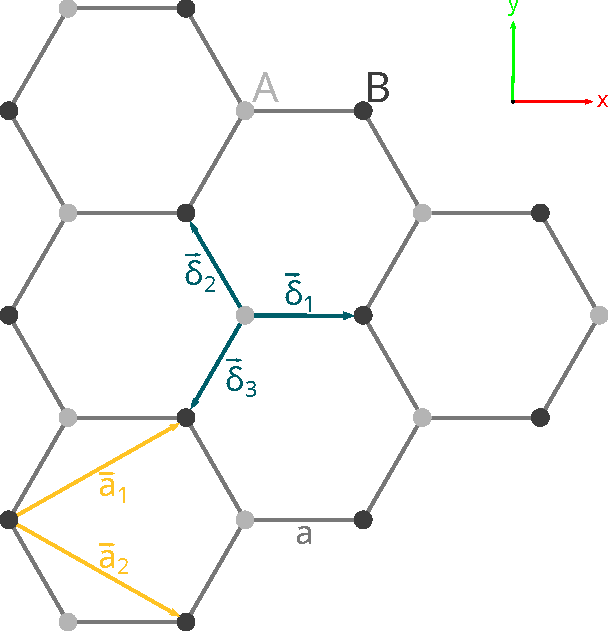
\includegraphics[width = 0.96 \textwidth]{Plots/graphene_lattice.pdf}
      \column{0.45\linewidth}
      \begin{itemize}
        \item Unterteilung in zwei Untergitter (A und B)
        \begin{itemize}
          \item[\textrightarrow] zweidimensionales, hexagonales Bravais-Gitter 
        \end{itemize}
        \item typische Honigwabenstruktur
        \item nächste-Nachbar Abstandsvektoren:
      \begin{equation*}
        \vec{\delta}_1 = a \begin{pmatrix} 1            \\[4pt] 0                   \end{pmatrix}, \quad
        \vec{\delta}_2 = a \begin{pmatrix} -\frac{1}{2} \\[4pt] \frac{\sqrt{3}}{2}  \end{pmatrix}, \quad 
        \vec{\delta}_3 = a \begin{pmatrix} -\frac{1}{2} \\[4pt] -\frac{\sqrt{3}}{2} \end{pmatrix} \label{eqn:nnvec}
    \end{equation*}
  \end{itemize}
  \end{columns}
\end{frame}
\begin{frame}{Struktur von Graphen und der Störstelle}
\begin{columns}
    \column{0.5\linewidth}
    \begin{figure}
      \centering
      \subfloat{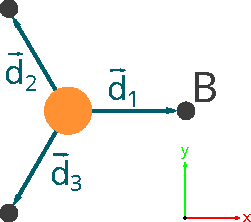
\includegraphics[height=2cm]{Plots/mangan_impurity_inplane.pdf}}\qquad
      \subfloat{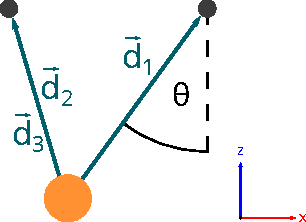
\includegraphics[height=2cm]{Plots/mangan_impurity_z_component.pdf}}
    \end{figure}
    \begin{equation*}
      \vec{d}_1 = a \begin{pmatrix} 1            \\[4pt] 0                   \\[2pt] \cot (\theta)\end{pmatrix}, \quad
      \vec{d}_2 = a \begin{pmatrix} -\frac{1}{2} \\[4pt] \frac{\sqrt{3}}{2}  \\[2pt] \cot (\theta)\end{pmatrix}, \quad 
      \vec{d}_3 = a \begin{pmatrix} -\frac{1}{2} \\[4pt] -\frac{\sqrt{3}}{2} \\[2pt] \cot (\theta)\end{pmatrix} 
    \end{equation*}
    \begin{itemize}
      \item Annahme: Mn mittig von den drei umliegenden C
      \item spiegelsymmetrisch um Graphenebene 
      \begin{itemize}
        \item[\textrightarrow] irrelevant, ob negative oder positive $z$-Komponente
      \end{itemize}
      \item Höhe des Mn variabel
    \end{itemize}
    \pause
    \column{0.5\linewidth}
    \vspace*{1cm}
    \centering
    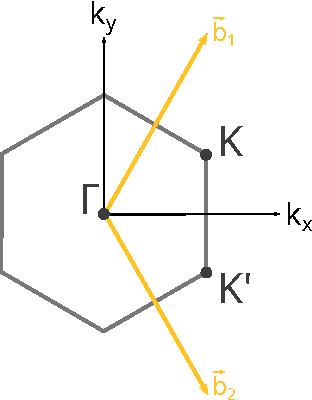
\includegraphics[width=3cm]{Plots/graphene_first_brillouine_zone.pdf}
    \vspace*{-0.2cm}
    \begin{itemize}
      \item reziprokes Gitter = um $90°$ gedrehtes hexagonales Gitter 
      \item Dirac-Punkte bei
    \begin{equation*}
      \vec{K}  = \frac{2\pi}{3\sqrt{3}a} \begin{pmatrix}  \sqrt{3}\\[4pt]  1   \end{pmatrix}, \quad
      \vec{K}' = \frac{2\pi}{3\sqrt{3}a} \begin{pmatrix}  \sqrt{3}\\[4pt]  -1  \end{pmatrix} 
    \end{equation*}
  \end{itemize}
\end{columns} 
\end{frame}

\begin{frame}{Eigenschaften von Graphen}
\begin{columns}
  \column{0.65\linewidth}
  \begin{itemize}
      \item $sp^2$-Hybridorbitale {\color{tugreen} \textrightarrow} $\sigma$-Bindung 
      \item $p$-Orbtiale {\color{tugreen} \textrightarrow} $\pi$-Bindung
      \end{itemize}
  \column{0.35\linewidth}
  \centering
    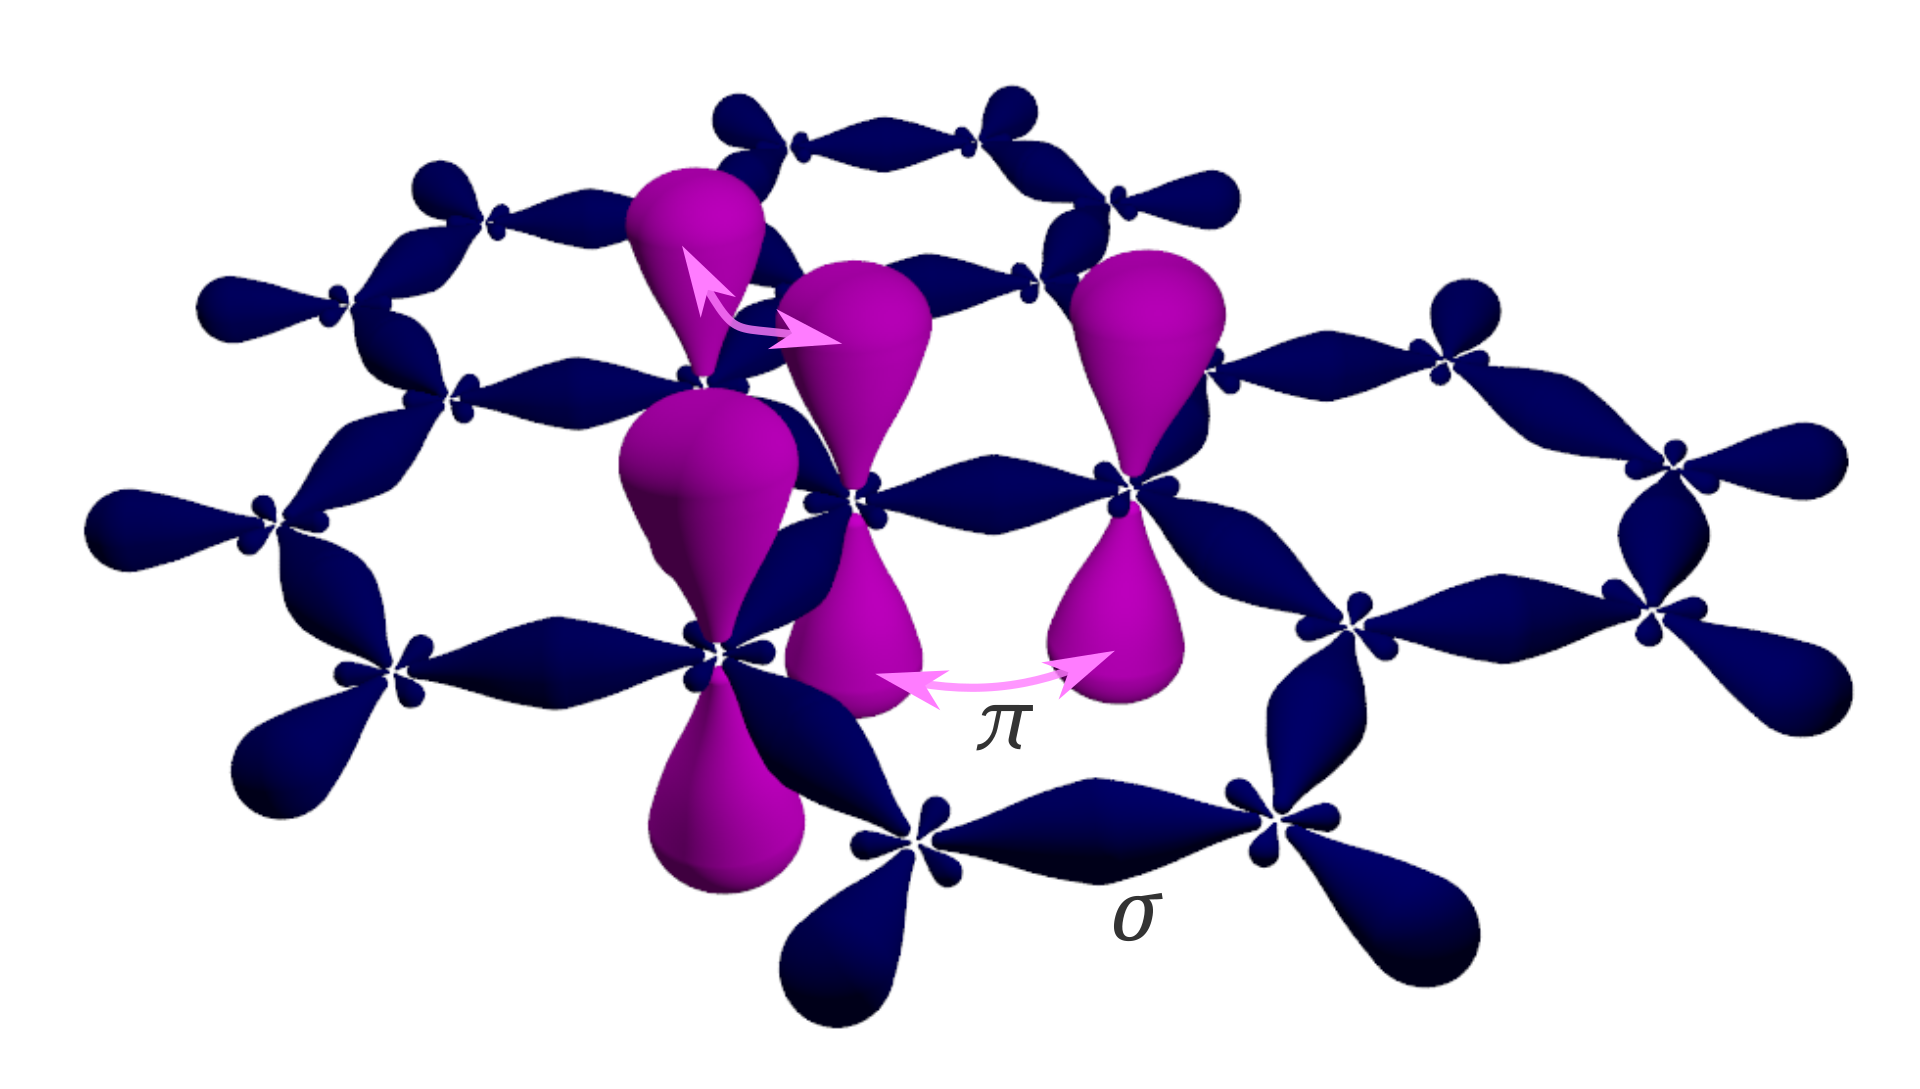
\includegraphics[width=\textwidth]{Plots/orbitals.png}
    \hspace*{12pt}\hbox{\scriptsize {\footnotesize\itshape \href{https://en.wikipedia.org/wiki/Graphene}{wikipedia.org/wiki/Graphene}}}
  \end{columns}
  \begin{columns}
  \column{0.65\linewidth}
  \pause 
  \begin{itemize}
    \vspace*{-2cm}
      \item 
      $\varepsilon_{\vec{k}} \propto \pm \sqrt{3+2 \cos \left ( \sqrt{3}ak_y \right )+2\cos \left ( \frac{3}{2}ak_x+\frac{\sqrt{3}}{2}ak_y \right ) + 2\cos \left ( \frac{3}{2}ak_x-\frac{\sqrt{3}}{2}ak_y \right ) }$
    \item Dispersionsrelation um Dirac-Punkte entwickeln
      \begin{itemize}
        \item[\textrightarrow] $\varepsilon_{\vec{k}} \propto \pm | \vec{k} |$
      \end{itemize}
    \end{itemize} 
    \column{0.35\linewidth}
    \vspace*{0.3cm}
    \centering
      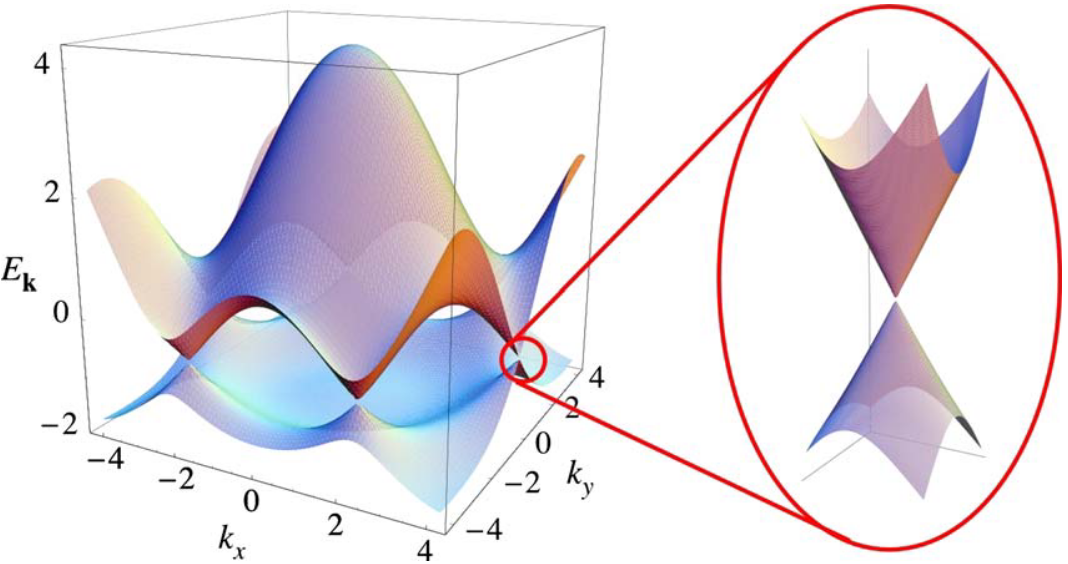
\includegraphics[width=\textwidth]{Plots/dirac_cones.png}
      \hspace*{12pt}\hbox{\scriptsize {\footnotesize\itshape \href{https://journals.aps.org/rmp/abstract/10.1103/RevModPhys.81.109}{A. H. Castro Neto et al., \textit{Rev. Mod. Phys.} 81 (2009)}}}
      % 10.1103/RevModPhys.81.109 (2009)
  \end{columns}
\end{frame}

\section{Theoretische Grundlagen}
\begin{frame}{Greensche Funktionen}
  \begin{itemize}
    \setlength\itemsep{1em}
  \item zwei Operatoren mit zeitl. Entwicklung  $ A \left ( \tau \right ) = \symup{e}^{H \tau} A_\text{S} \symup{e}^{-H \tau} $ und  
  $ B \left ( \tau' \right ) = \symup{e}^{H \tau'} B_\text{S} \symup{e}^{-H \tau'}$
  \item Greensche Funktion $G_{A,B} \left (\tau, \tau' \right ) = -\langle T_s \left ( A \left (\tau \right ) B \left ( \tau' \right ) \right ) \rangle
  = -  \left(  \langle A \left (\tau \right ) B \left ( \tau' \right ) \rangle \symup{\Theta} \left ( \tau - \tau' \right) + s 
  \langle B \left ( \tau' \right ) A \left (\tau \right ) \rangle \symup{\Theta} \left ( \tau' - \tau \right)  \right )$
  \item Bewegungsgleichung $\frac{\partial}{\partial \tau} G_{A,B} \left (\tau, \tau' \right) = G_{[H,A],B}(\tau, \tau') - \langle \{ A,B \} \rangle \delta \left ( \tau - \tau' \right) $
  \item Fourier-transformierte Bewegungsgleichung $\boxed{zG_{A,B}(z) = \langle \{A,B\} \rangle - G_{[H,A],B}(z)}$
\end{itemize}  
\end{frame}

\begin{frame}{Tight Binding Modell}
  \begin{itemize}
    \setlength\itemsep{0.8em}
    \item Ausgang: stark gebundene, lokalisierte Elektronen mit Wellenfunktionen $\Psi_{lm}(\vec{r}-\vec{l}_j - \vec{R}_{\alpha})$
    \item Betrachtung des Hamiltonians für ein Elektron $H = \frac{\vec{p}^2}{2M} + \sum_{j\alpha} v(\vec{r}-\vec{l}_j - \vec{R}_{\alpha}) = \frac{\vec{p}^2}{2M} + v_{\vec{R}}(\vec{r})$
    \item Dreizentren-Beiträge vernachlässigen, da Elektronen stark lokalisiert sind
    \begin{itemize}
      \item[\textrightarrow] $\boxed{t^{j\alpha,j'\alpha'}_{lm,l'm'} = - \int \symup{d}^3r \; \overline{\Psi}_{lm} \left (\vec{r}-\vec{l}_j - \vec{R}_{\alpha} \right ) 
      v \left ( \vec{r} - \vec{l}_{j} - \vec{R}_{\alpha} \right ) \Psi_{l'm'} \left (\vec{r}-\vec{l}_{j'} - \vec{R}_{\alpha'} \right )}$
    \end{itemize}
    \item Tight Binding Hamiltonian in zweiter Quantisierung $H = - \sum_{jj'} \sum_{\alpha \alpha'}\sum_{ll'} \sum_{mm'} t^{j\alpha,j'\alpha'}_{lm,l'm'}  c_{jlm\alpha}^\dagger c_{j'l'm'\alpha'}$
  \end{itemize}
\end{frame}

\begin{frame}{Slater-Koster-Integrale}
  \begin{equation*}
    \boxed{E_{lm,l'm'} = \int \symup{d}^3r \; \overline{\Psi}_{lm} \left (\vec{r}-\vec{d} \, \right )
    V \left ( \vec{r} - \vec{d} \, \right ) \Psi_{l'm'} \left (\vec{r} \right )}
  \end{equation*}
  \begin{itemize}
    \item SK-Integrale als Bestimmung der Hüpfmatrixelemente
    \item hängen nur vom Abstand ab 
    \item Unterteilung in SK-Integrale zu den zugehörigen Symmetrien $V_{ll'\eta}$
    \item im Allgemeinen Aufteilung der SK-Integrale in die einzelnen Integrale $V_{ll'\eta}$ mit Richtungskosinus als Vorfaktoren
  \end{itemize}
  \begin{equation*}
    l = \frac{\vec{d} \cdot \hat{x}}{\left | \vec{d} \right |} \; , \quad
    m = \frac{\vec{d} \cdot \hat{y}}{\left | \vec{d} \right |} \; , \quad
    n = \frac{\vec{d} \cdot \hat{z}}{\left | \vec{d} \right |} \label{eqn:RK}
\end{equation*}\\
\vspace*{0.45cm}
\begin{flushleft}
Beispiel: $E_{z,x^2-y^2} = \frac{\sqrt{3}}{2}n(l^2-m^2) V_{pd\sigma} - n (l^2-m^2) V_{pd\pi}$ 
\end{flushleft}
\pause
\vspace*{1.67cm}
\begin{tikzpicture}[remember picture,overlay]
\node at (current page.center) {\colorbox{white}{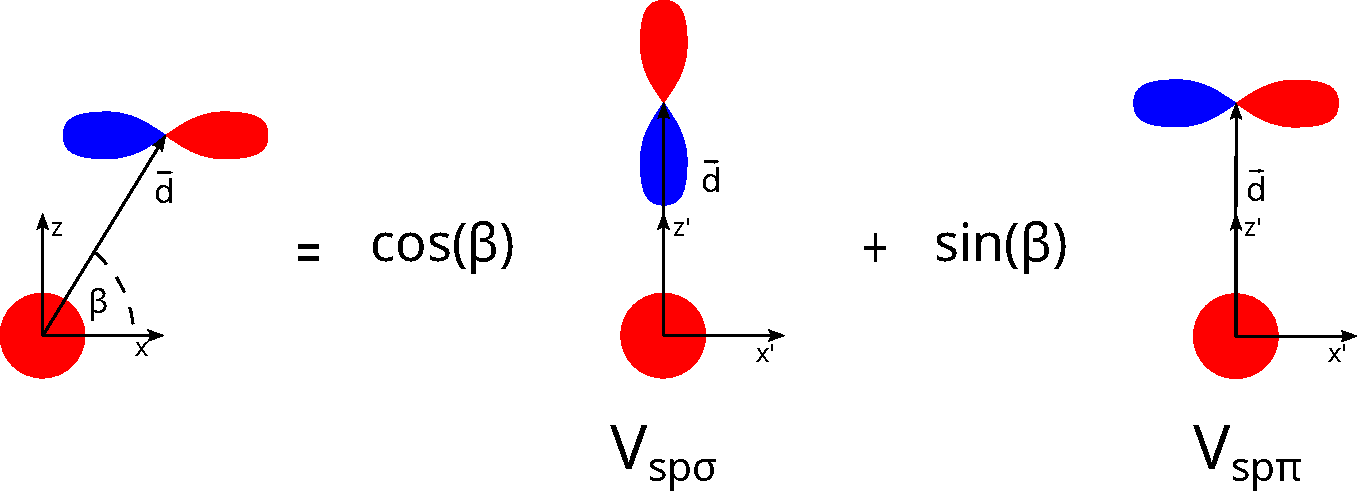
\includegraphics[width = 0.9\textwidth, center]{Plots/SK.pdf}}};
\end{tikzpicture}
\vspace*{-1.2cm}
\begin{equation*}
  E_{s,x} = lV_{pd\sigma}
\end{equation*}
\end{frame}

\section{Ergebnisse}
\begin{frame}{Hamiltonian des gesamten Systems}
  \vspace*{-0.2cm}
  \huge
  \begin{equation*}
    H =   H_0 +  H_\text{Def}  +  H_\text{Kop}
  \end{equation*}
  \normalsize
  \pause
  \vspace*{0.35cm}
  \begin{equation*}
    H = \underbrace{- t  \sum_{i=1}^N \sum_{j=1}^3
    \left ( c_{\text{A},\vec{l}_i}^\dagger c_{\text{B},\vec{l}_i+\vec{\delta}_j} + c_{\text{B},\vec{l}_i+\vec{\delta}_j}^\dagger c_{\text{A},\vec{l}_i} \right )}_{\mathlarger{H_0}} \Pause 
    + \underbrace{\sum_{m=1}^5 \varepsilon_m d^\dagger_m d_m}_{\mathlarger{H_\text{Def}}}  \Pause
    + \underbrace{\sum_{m=1}^5 \sum_{j=1}^3 \left ( V_{mj} d_m^\dagger c_{\text{B},\vec{l}+\vec{\delta}_j} + \overline{V}_{mj} c_{\text{B},\vec{l}+\vec{\delta}_j}^\dagger d_m \right ) }_{\mathlarger{H_\text{Kop}}}
  \end{equation*}
\end{frame}

\begin{frame}{Ermittelte Slater-Koster-Integrale}
  \begin{table}
    \centering
    \begin{tabular}{l c c c}
    & \multicolumn{3}{c}{$j$-tes C}\\
    \cmidrule(lr){2-4}
    & {$1$} & {$2$} & {$3$} \\
    \midrule
    {$E_{z,xy}$      }  & {$\color{Apricot}0$}                                               & {$\color{Apricot}-\frac{3}{4}bV_{pd\sigma} + \frac{\sqrt{3}}{2}bV_{pd\pi}$}          & {$\color{Apricot} \frac{3}{4}bV_{pd\sigma}-\frac{\sqrt{3}}{2}bV_{pd\pi}$}         \vspace{0.5cm} \\ 
    {$E_{z,xz}$      }  & {$\color{Aquamarine}\sqrt{3}fV_{pd\sigma} + hV_{pd\pi}$}              & {$\color{Aquamarine}-\frac{\sqrt{3}}{2}fV_{pd\sigma} - \frac{1}{2} hV_{pd\pi}$}         & {$\color{Aquamarine}-\frac{\sqrt{3}}{2}fV_{pd\sigma} - \frac{1}{2} hV_{pd\pi}$}      \vspace{0.5cm} \\
    {$E_{z,zy}$      }  & {$\color{Aquamarine}0$}                                               & {$\color{Aquamarine} \frac{3}{2}fV_{pd\sigma}+\frac{\sqrt{3}}{2} hV_{pd\pi}$}           & {$\color{Aquamarine}-\frac{3}{2}fV_{pd\sigma}-\frac{\sqrt{3}}{2} hV_{pd\pi}$}        \vspace{0.5cm} \\
    {$E_{z,3z^2-r^2}$}  & {$\color{LimeGreen} q V_{pd\sigma}+\sqrt{3}bV_{pd\pi}$}               & {$\color{LimeGreen}q V_{pd\sigma}+\sqrt{3}bV_{pd\pi}$}                                 & {$\color{LimeGreen}q V_{pd\sigma}+\sqrt{3}bV_{pd\pi}$} \vspace{0.5cm} \\
    {$E_{z,x^2-y^2}$ }  & {$\color{Apricot}\frac{\sqrt{3}}{2}bV_{pd\sigma}-bV_{pd\pi}$}      & {$\color{Apricot}-\frac{\sqrt{3}}{4}bV_{pd\sigma}+\frac{1}{2}bV_{pd\pi}$}           & {$\color{Apricot}-\frac{\sqrt{3}}{4}bV_{pd\sigma}+\frac{1}{2}bV_{pd\pi}$}                       \\ 
    \bottomrule
    \end{tabular}
  \end{table}
  \vspace{0.3cm}
  \begin{equation*}
    \begin{aligned}
b & \coloneq -\sin^2(\theta) \cos(\theta)        & f &  \coloneq -\cos^2(\theta) \sin(\theta)                             \\                     
h & \coloneq -\sin(\theta)(1-2\cos^2(\theta))    & q &  \coloneq -\cos^3(\theta) + \frac{1}{2}\sin^2(\theta) \cos(\theta)
    \end{aligned} \label{eqn:Vorfaktoren}
\end{equation*}
\end{frame}
\begin{frame}{Hybridisierungsfunktion mittels Bewegungsleichungen}
\begin{equation*}
      H = -t \sum_{j \vec{k}} \left ( \symup{e}^{\symup{i}\vec{k}\vec{\delta}_j}c^\dagger_{\text{A},\vec{k}} c_{\text{B},\vec{k}} + 
      \symup{e}^{-\symup{i}\vec{k}\vec{\delta}_j} c^\dagger_{\text{B},\vec{k}}c_{\text{A},\vec{k}} \right ) + \sum_m \varepsilon_m d_m^\dagger d_m 
      + \frac{1}{\sqrt{N}}\sum_{mj\vec{k}} \left ( V_{mj}  \symup{e}^{\symup{i}\vec{k}(\vec{l}+\vec{\delta}_j)} d_m^\dagger c_{\text{B},\vec{k}} 
      + V_{mj} \symup{e}^{-\symup{i}\vec{k}(\vec{l}+\vec{\delta}_j)}c^\dagger_{\text{B},\vec{k}} d_m \right )
\end{equation*}
\vspace*{0.5cm}
\pause
Damit ergibt sich folgende Greensche Funktion  %$Erinnerung: zG_{A,B}(z) = \langle \{A,B\} \rangle - G_{[H,A],B}(z)$
\begin{equation*}
  \left (z-\varepsilon_m \right )G_{d_m, d_{m'}^\dagger} = \delta_{mm'} + \frac{1}{\sqrt{N}}\sum_{j\vec{k}} V_{mj} 
    \symup{e}^{\symup{i}\vec{k} (\vec{l} + \vec{\delta}_j)} G_{c_{\text{B},\vec{k}}, d^\dagger_{m'}}
\end{equation*}
\pause
\vspace*{-0.2cm}
\begin{equation*}
  \! \! \! \! \! \! \! \! \! \! \! \!   G_{c_{\text{B},\vec{k}}, d^\dagger_{m'}} =\frac{1}{z} \left (- t \sum_{j} \symup{e}^{-\symup{i}\vec{k} \vec{\delta}_j} G_{c_{\text{A},\vec{k}},d^\dagger_{m'}} + 
    \frac{1}{\sqrt{N}} \sum_{mj} V_{mj} \symup{e}^{-\symup{i}\vec{k} (\vec{l}+ \vec{\delta}_j)} G_{d_m, d_{m'}^\dagger} \right )\; \Pause , \quad \quad \quad \quad 
    G_{c_{\text{A},\vec{k}},d^\dagger_{m'}} = - \frac{t \sum_{j}\symup{e}^{\symup{i}\vec{k}\vec{\delta}_j} G_{c_{\text{B},\vec{k}}, d^\dagger_{m'}}} {z}
  \end{equation*}
\end{frame}
\begin{frame}{Hybridisierungsfunktion mittels Bewegungsleichungen}
\begin{equation*}
  \left (  \underline{\underline{G}}^{-1} \right )_{mn} = \left ( z- \varepsilon_m \right ) \delta_{mn} - \frac{z}{N}\sum_{\vec{k}}
    \frac{\sum_j V_{mj}\symup{e}^{\symup{i}\vec{k}\vec{\delta}_j}\sum_{j'} V_{nj'}\symup{e}^{-\symup{i}\vec{k}\vec{\delta}_{j'}}}
    {z^2-\varepsilon_{\vec{k}}^2}
\end{equation*}
Struktur von $\underline{\underline{G}}^{-1}$
\begin{equation*}
  \underline{\underline{G}}^{-1} = \underline{\underline{Z}} - \underline{\underline{E}} - \underline{\underline{\symup{\Delta}}}
\end{equation*}
Die gesuchte Hybridisierungsfunktion ist gegeben durch
\begin{equation*}
  \boxed { \left ( \,  \underline{\underline{\symup{\Delta}}}  \, \right )_{mn} =  \frac{z}{N}\sum_{\vec{k}}
    \frac{\sum_j V_{mj}\symup{e}^{\symup{i}\vec{k}\vec{\delta}_j}\sum_{j'} V_{nj'}\symup{e}^{-\symup{i}\vec{k}\vec{\delta}_{j'}}}
    {z^2-\varepsilon_{\vec{k}}^2} }
\end{equation*}
\end{frame}

\begin{frame}{Hybridisierungsfunktion mittels Basistransformation}
\vspace*{1cm}
Basistransformation 
\begin{columns}
  \begin{column}{0.4 \linewidth}
  \begin{align*}
    \tilde{c}_0 &= \frac{1}{\sqrt{3}}\left (c_{\text{B},\vec{l}+\vec{\delta}_1} + c_{\text{B},\vec{l}+\vec{\delta}_2} + c_{\text{B},\vec{l}+\vec{\delta}_3} \right ) \\
    \tilde{c}_1 &= \frac{1}{\sqrt{3}}\left (c_{\text{B},\vec{l}+\vec{\delta}_1}+ \symup{e}^{\symup{i}\frac{2\pi}{3}} c_{\text{B},\vec{l}+\vec{\delta}_2} + \symup{e}^{\symup{i}\frac{4\pi}{3}}c_{\text{B},\vec{l}+\vec{\delta}_3} \right ) \\
    \tilde{c}_2 &= \frac{1}{\sqrt{3}}\left (c_{\text{B},\vec{l}+\vec{\delta}_1} + \symup{e}^{\symup{i}\frac{4\pi}{3}} c_{\text{B},\vec{l}+\vec{\delta}_2} + \symup{e}^{\symup{i}\frac{2\pi}{3}}c_{\text{B},\vec{l}+\vec{\delta}_3} \right )
    \end{align*}
  \end{column}
    \begin{column}{0.1 \linewidth}
      \vspace{-0.3cm}
      \huge $\iff$
  \end{column}
    \begin{column}{0.3 \linewidth}
    \begin{align*}
      \!  \! \! \! \!  \! \! \! \! \! \! \! \! c_{\text{B},\vec{l}+\vec{\delta}_1} &= \frac{1}{\sqrt{3}}\left (\tilde{c}_0 + \tilde{c}_1 + \tilde{c}_2 \right ) \\
      c_{\text{B},\vec{l}+\vec{\delta}_2} &= \frac{1}{\sqrt{3}}\left (\tilde{c}_0 + \symup{e}^{\symup{i}\frac{4\pi}{3}} \tilde{c}_1 + \symup{e}^{\symup{i}\frac{2\pi}{3}} \tilde{c}_2 \right ) \\
      c_{\text{B},\vec{l}+\vec{\delta}_3} &= \frac{1}{\sqrt{3}}\left (\tilde{c}_0 + \symup{e}^{\symup{i}\frac{2\pi}{3}} \tilde{c}_1 + \symup{e}^{\symup{i}\frac{4\pi}{3}} \tilde{c}_2 \right )   
    \end{align*}
    \end{column}
    \end{columns}
    \vspace*{0.7cm}
    \begin{equation*}
      H_\text{Kop} = \sum_{m=1}^5 \sum_{j=1}^3 \left ( V_{mj} d_m^\dagger c_{\text{B},\vec{l}+\vec{\delta}_j} + \overline{V}_{mj} c_{\text{B},\vec{l}+\vec{\delta}_j}^\dagger d_m \right )
      \end{equation*}
    \end{frame}
    \begin{frame}{Hybridisierungsfunktion mittels Basistransformation}
\begin{align*}
  H_\text{Kop} = \frac{1}{\sqrt{3}} 
      \Biggl(  &\left ( \left   ({\color{Apricot}-\frac{3}{4}\sqrt{3}    b   V_{pd\sigma} + \frac{3}{2}     b   V_{pd\pi}  } \right ) \tilde{c}^\dagger_1  
                  +\left  ( {\color{Apricot} \frac{3}{4}\sqrt{3}       b   V_{pd\sigma} - \frac{3}{2}     b   V_{pd\pi} } \right ) \tilde{c}^\dagger_2 \right )             \symup{i}  d_1\\
      +&\left (    \left  ( {\color{Aquamarine}\frac{3}{2}\sqrt{3}                           f   V_{pd\sigma} + \frac{3}{2}              h   V_{pd\pi} } \right ) \tilde{c}^\dagger_1          
                  +\left  ( {\color{Aquamarine}\frac{3}{2}\sqrt{3}                           f   V_{pd\sigma} + \frac{3}{2}              h   V_{pd\pi} }\right ) \tilde{c}^\dagger_2 \right ) d_2\\
      +&\left (    \left  ( {\color{Aquamarine}\frac{3}{2}\sqrt{3}                  f   V_{pd\sigma} + \frac{3}{2}     h   V_{pd\pi} }\right ) \tilde{c}^\dagger_1  
                  +\left  ({\color{Aquamarine}-\frac{3}{2}\sqrt{3}                  f   V_{pd\sigma} - \frac{3}{2}     h   V_{pd\pi} }\right ) \tilde{c}^\dagger_2 \right )  \symup{i}  d_3\\
      +&\left (   { \color{LimeGreen}3 q V_{pd\sigma} + 3 \sqrt{3}  b V_{pd\pi} } \right )    \tilde{c}^\dagger_0                                                                              d_4\\
      +&\left (   \left   ( {\color{Apricot}\frac{3}{4}\sqrt{3}                           b   V_{pd\sigma} - \frac{3}{2}              b   V_{pd\pi} } \right ) \tilde{c}^\dagger_1  
                  +\left  ( { \color{Apricot} \frac{3}{4}\sqrt{3}                           b   V_{pd\sigma} - \frac{3}{2}              b   V_{pd\pi} } \right ) \tilde{c}^\dagger_2 \right ) d_5 \Biggr) \\
                  &  \!  \! \! \! \!  \! \! \! \! \! \! \! \! + \text{h.c.}
\end{align*}
\begin{align*}
  \tilde{d}_0 &= \frac{1}{\sqrt{2}} (d_5-\symup{i}d_1) &     {\color{Periwinkle}  d_{x^2-y^2}, \; d_{xy}}  \quad \quad \quad \quad \quad \quad \quad \quad \quad \quad \tilde{d}_2 &= \frac{1}{\sqrt{2}} (d_5+\symup{i}d_1) \\
  \tilde{d}_1 &= \frac{1}{\sqrt{2}} (d_2+\symup{i}d_3) &     {\color{Periwinkle}  d_{xz},      \; d_{zy}}  \; \; \quad \quad \quad \quad \quad \quad \quad \quad \quad \quad \tilde{d}_3 &= \frac{1}{\sqrt{2}} (d_2-\symup{i}d_3)
  \end{align*}
  %\begin{align*}
  \end{frame}
  \begin{frame}{Hybridisierungsfunktion mittels Basistransformation}
%    \begin{wrapfigure}{r}{0.3\textwidth}
%      \centering
%      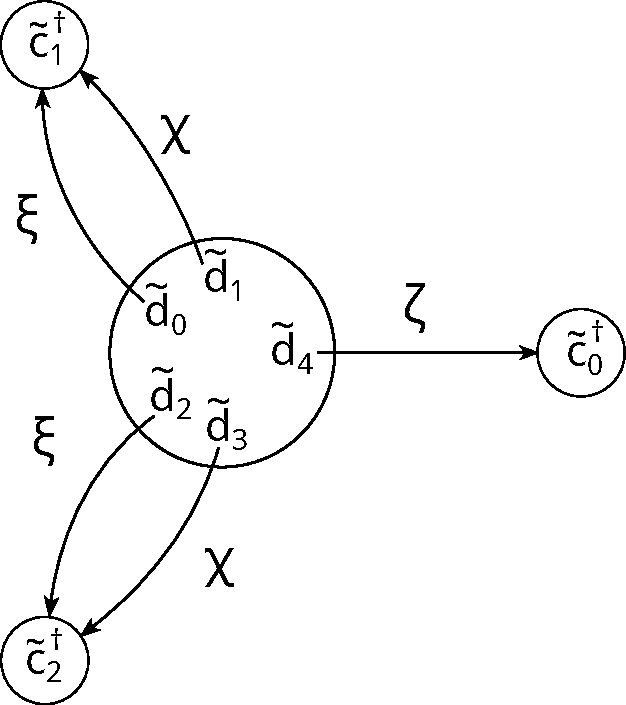
\includegraphics[width = 0.25\textwidth]{Plots/3band.pdf}
%    \end{wrapfigure}
\begin{columns}
  \column{0.7\linewidth} 
  \mathleft
    \begin{equation*}
      \text{Erinnerung: } H_\text{Kop} = \sum_{m=1}^5 \sum_{j=1}^3 \left ( V_{mj} d_m^\dagger c_{\text{B},\vec{l}+\vec{\delta}_j} + \overline{V}_{mj} c_{\text{B},\vec{l}+\vec{\delta}_j}^\dagger d_m \right )
    \end{equation*}
    \mathcenter
    \vspace*{1cm}
    \begin{empheq}[box=\widefbox]{equation*}
     H_\text{Kop} = 
        \xi \left ( \tilde{d}^\dagger_0 \tilde{c}_1 + \tilde{d}^\dagger_2 \tilde{c}_2 \right )
    +   \chi \left ( \tilde{d}^\dagger_1 \tilde{c}_1 + \tilde{d}^\dagger_3 \tilde{c}_2 \right )  
    +   \zeta \, \tilde{d}^\dagger_4 \tilde{c}_0 + \text{h.c.}
  \end{empheq}
%\vspace*{0.05cm}
\begin{center}
 \color{tugreen} \huge \textbf{Effektives Drei-Bänder Modell} 
\end{center}
\column{0.3\linewidth}
\hspace{-0.7cm}
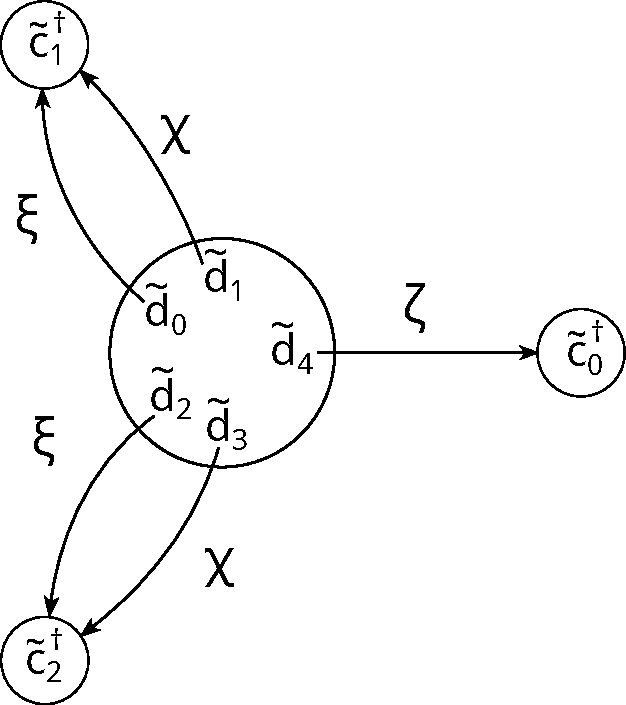
\includegraphics[width=\textwidth]{Plots/3band.pdf}
\end{columns}
\vspace*{1cm}
\begin{equation*}
  \xi = \left ( {\color{Apricot}\frac{3}{\sqrt{8}} b V_{pd\sigma} - \frac{\sqrt{3}}{\sqrt{2}}  b   V_{pd\pi} }\right ) \, , 
  \quad \chi = \left ( { \color{Aquamarine} \frac{3}{\sqrt{2}} f V_{pd\sigma} + \frac{\sqrt{3}}{\sqrt{2}}  h   V_{pd\pi} } \right ) \, ,
  \quad \zeta = \left ( {\color{LimeGreen} \sqrt{3} q V_{pd\sigma} + 3 b V_{pd\pi} } \right )
\end{equation*}
\end{frame}
\begin{frame}{Hybridisierungsfunktion mittels Basistransformation}
\vspace*{0.3cm}
  \begin{equation*}
  H = -t\sum_{i=1}^N \sum_{j=1}^3 \left ( c_{\text{A},\vec{l}_i}^\dagger c_{\text{B},\vec{l}_i+\vec{\delta}_j} + 
  c_{\text{B},\vec{l}_i+\vec{\delta}_j}^\dagger c_{\text{A},\vec{l}_i} \right ) + \varepsilon \sum_{m=0}^4 \tilde{d}^\dagger_m \tilde{d}_m
  +\sum_{m=0}^4\sum_{l=0}^2 \left (\gamma_{ml} \tilde{d}^\dagger_m \tilde{c}_l + \gamma_{ml} \tilde{c}^\dagger_l \tilde{d}_m \right )
\end{equation*}
\begin{wrapfigure}{r}{0.3\textwidth}
  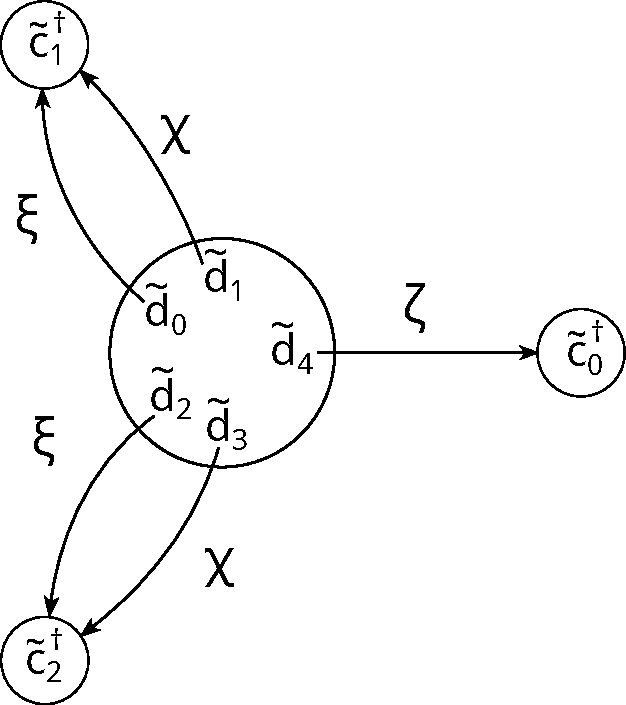
\includegraphics[width = 0.3\textwidth]{Plots/3band.pdf}
\end{wrapfigure}
\vspace*{1cm}
\begin{equation*}
  \underline{\underline{\gamma}} = 
  \begin{pmatrix}
  0               & \xi    &   0           \\
  0               & \chi   &   0           \\
  0               & 0             &   \xi \\
  0               & 0             &   \chi \\
  \zeta     & 0             &   0           \\
\end{pmatrix}
\end{equation*}
\begin{itemize}
  \item Die Struktur der Hybridisierungsfunktion $\underline{\underline{\symup{\Delta}}}$ kann direkt abgelesen werden
  \begin{itemize}
    \item[\textrightarrow] $\underline{\underline{\symup{\Delta}}}$ wird eine blockdiagonale Struktur mit zwei $2 \times 2$-Blöcken und \\ einem  $ 1 \times 1$-Block haben
  \end{itemize}
\end{itemize}
\end{frame}
\begin{frame}{Hybridisierungsfunktion mittels Basistransformation}
\[  \def\spacednull{\rlap{0}\phantom{\gamma_{01}^2\gamma_{11}}}
    \def\nullblock{\begin{matrix}\spacednull&\spacednull\\\spacednull&\spacednull\end{matrix}}
    \def\nullrow{\begin{matrix}\spacednull&\spacednull\end{matrix}}
     \underline{\underline{\symup{\Delta}}} = 
\begin{pmatrix}
    \begin{pmatrix}
        \xi^2           & \xi \chi                \\
        \xi\chi  & \chi^2                         \\
    \end{pmatrix} G_{\tilde{c}_1, \tilde{c}^\dagger_1}   &   \nullblock  &   \begin{matrix}0\\0\end{matrix}            \\
    \nullblock      & \begin{pmatrix}
                        \xi^2           & \xi\chi\\
                        \xi\chi  & \chi^2         \\
                      \end{pmatrix} G_{\tilde{c}_2, \tilde{c}^\dagger_2}  &   \begin{matrix}0\\0\end{matrix}          \\
    \nullrow      &   \nullrow  &   \zeta^2           G_{\tilde{c}_0, \tilde{c}^\dagger_0}       \\
\end{pmatrix}
\]
\begin{itemize}
  \item $G_{\tilde{c}_l, \tilde{c}^\dagger_l}$ über Rücktransformation von $G_{c_{\text{B},\vec{k}}, c^\dagger_{\text{B},\vec{k}}}$ bestimmen
  \item $G_{c_{\text{B},\vec{k}}, c^\dagger_{\text{B},\vec{k}}}$ des ungestörten Graphens benutzen
  \begin{itemize}
    \item Einfluss des Mn geht für große Systemgrößen gegen 0 
  \end{itemize} 
\end{itemize}
\mathleft
\vspace*{1.4cm}
\begin{equation*}
  \text{Erinnerung: }H_0 = - t  \sum_{i=1}^N \sum_{j=1}^3
    \left ( c_{\text{A},\vec{l}_i}^\dagger c_{\text{B},\vec{l}_i+\vec{\delta}_j} + c_{\text{B},\vec{l}_i+\vec{\delta}_j}^\dagger c_{\text{A},\vec{l}_i} \right ) 
    = -t \sum_{j \vec{k}} \left ( \symup{e}^{\symup{i}\vec{k}\vec{\delta}_j}c^\dagger_{\text{A},\vec{k}} c_{\text{B},\vec{k}} + 
    \symup{e}^{-\symup{i}\vec{k}\vec{\delta}_j} c^\dagger_{\text{B},\vec{k}}c_{\text{A},\vec{k}} \right )
\end{equation*}
\end{frame}
\begin{frame}{Hybridisierungsfunktion mittels Basistransformation}
\mathcenter
\begin{equation*}
  G_{c_{\text{B},\vec{k}}, c^\dagger_{\text{B},\vec{k}}} = \frac{z}{z^2 - \varepsilon^2_{\vec{k}}  } \quad
  \implies \quad G_{\tilde{c}_l, \tilde{c}^\dagger_{l'}} = \sum_{\vec{k}} D_{l,\vec{k}} D^\dagger_{l',\vec{k}}G_{c_{\text{B},\vec{k}}, c^\dagger_{\text{B},\vec{k}}}
\end{equation*}
\vspace*{0.5cm}
Die Koeffizienten $D_{l,\vec{k}}$ können von den Fouriertransformationen für $\tilde{c}_l$ abgelesen werden
\pause
\vspace*{0.5cm}
\begin{equation*}
    \tilde{c}_0 =   \frac{1}{\sqrt{3N}}\sum_{\vec{k}} \sum_{j=1}^3\symup{e}^{\symup{i}{\vec{k}}(\vec{l}+\vec{\delta}_j)}                            c_{\text{B}, \vec{k}} \; , \quad
    \tilde{c}_1 = \frac{1}{\sqrt{3N}}\sum_{\vec{k}} \sum_{j=1}^3\symup{e}^{\symup{i}{\vec{k}}(\vec{l}+\vec{\delta}_j)+\symup{i}\frac{2(j-1)\pi}{3}} c_{\text{B}, \vec{k}} \; , \quad
    \tilde{c}_2 = \frac{1}{\sqrt{3N}}\sum_{\vec{k}} \sum_{j=1}^3\symup{e}^{\symup{i}{\vec{k}}(\vec{l}+\vec{\delta}_j)-\symup{i}\frac{2(j-1)\pi}{3}} c_{\text{B}, \vec{k}}
\end{equation*}
\pause
\vspace*{0.1cm}
\begin{equation*}
    G_{\tilde{c}_0, \tilde{c}^\dagger_0} = \frac{z}{3N} \sum_{\vec{k}} \frac{\sum_j \symup{e}^{\symup{i}{\vec{k}}\vec{\delta}_j} \sum_{j'} \symup{e}^{-\symup{i}{\vec{k}}\vec{\delta}_{j'}}                                                            }{z^2-\varepsilon_{\vec{k}}^2} \; , \quad
    G_{\tilde{c}_1, \tilde{c}^\dagger_1} = \frac{z}{3N} \sum_{\vec{k}} \frac{\sum_j \symup{e}^{\symup{i}{\vec{k}}\vec{\delta}_j+\symup{i}\frac{2(j-1)\pi}{3}} \sum_{j'} \symup{e}^{-\symup{i}{\vec{k}}\vec{\delta}_{j'}-\symup{i}\frac{2(j'-1)\pi}{3}} }{z^2-\varepsilon_{\vec{k}}^2} \; , \quad
    G_{\tilde{c}_2, \tilde{c}^\dagger_2} = \frac{z}{3N} \sum_{\vec{k}} \frac{\sum_j \symup{e}^{\symup{i}{\vec{k}}\vec{\delta}_j-\symup{i}\frac{2(j-1)\pi}{3}} \sum_{j'} \symup{e}^{-\symup{i}{\vec{k}}\vec{\delta}_{j'}+\symup{i}\frac{2(j'-1)\pi}{3}} }{z^2-\varepsilon_{\vec{k}}^2}
\end{equation*}
\end{frame}
\begin{frame}{Hybridisierungsfunktion mittels Basistransformation}
\[  \def\spacednull{\rlap{0}\phantom{\gamma_{01}^2\gamma_{11}}}
    \def\nullblock{\begin{matrix}\spacednull&\spacednull\\\spacednull&\spacednull\end{matrix}}
    \def\nullrow{\begin{matrix}\spacednull&\spacednull\end{matrix}}
          \colorlet{oldcolor}{.}
     \color{red}
     \boxed { \color{oldcolor}
     \underline{\underline{\symup{\Delta}}} =  
    \begin{pmatrix}
    \begin{pmatrix}
        \xi^2           & \xi \chi                \\
        \xi\chi  & \chi^2                         \\
    \end{pmatrix} G_{\tilde{c}_1, \tilde{c}^\dagger_1}   &   \nullblock  &   \begin{matrix}0\\0\end{matrix}            \\
    \nullblock      & \begin{pmatrix}
                        \xi^2           & \xi\chi\\
                        \xi\chi  & \chi^2         \\
                      \end{pmatrix} G_{\tilde{c}_2, \tilde{c}^\dagger_2}  &   \begin{matrix}0\\0\end{matrix}          \\
    \nullrow      &   \nullrow  &   \zeta^2           G_{\tilde{c}_0, \tilde{c}^\dagger_0}       \\
\end{pmatrix} }
\]
\end{frame}

\begin{frame}{Einfluss der Höhe $z$ des Mn}
\centering
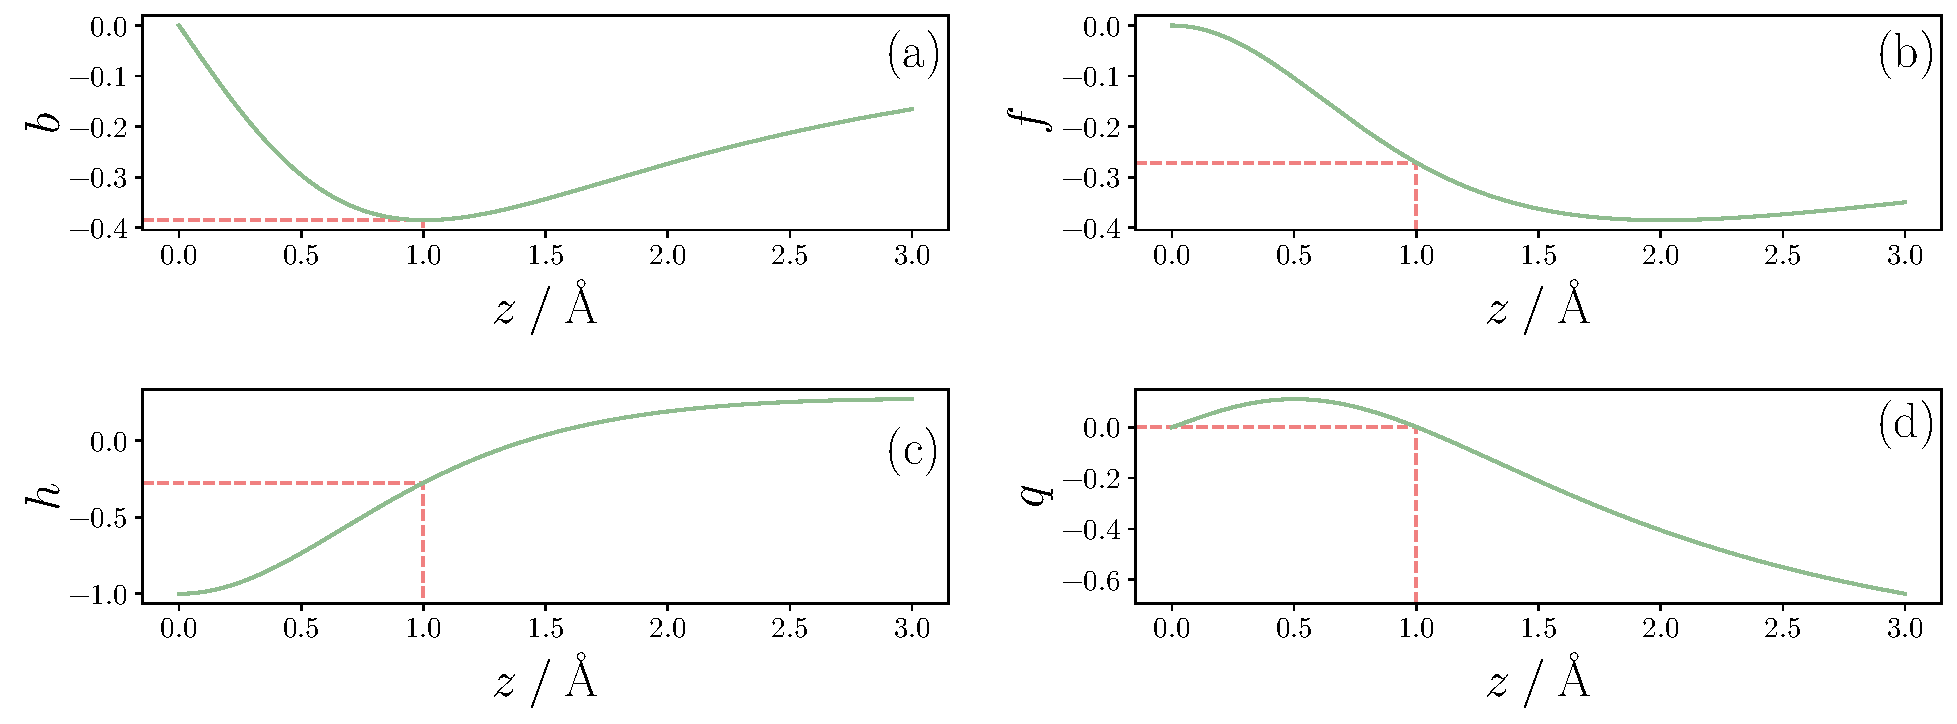
\includegraphics[width = 0.95\textwidth]{Plots/Faktoreninz.pdf}
\begin{itemize}
  \item $b$ klein bei geringen Höhen            $\color{tugreen}\to$ $E_{z,xy}$ und $E_{z,x^2-y^2}$ verschwinden
  \item $h$ klein bei großen Höhen            $\color{tugreen}\to$ $V_{pd\pi}$ geringen Einfluss bei $E_{z,xz}$und $E_{z,zy}$
  \item $q=0$ bei genau $z=\qty{1}{\angstrom}$  $\color{tugreen}\to$ $V_{pd\sigma}$ kein Einfluss bei $E_{z,3z^2-r^2}$
\end{itemize}
\end{frame}
\section{Zusammenfassung und Ausblick}
\begin{frame}{Zusammenfassung und Ausblick}
  \begin{columns}
    \column{0.7\linewidth}
  \begin{itemize}[<+->]
    \item Hybridisierungsfunktion in neuer Basis in irreduzible Blöcke zerfallen
    \item effektives Drei-Bänder Modell für Ankopplung der $3d$-Orbitale an Graphenbandstruktur
    \item Diskussions der Höhe des Mn
    \vspace*{0.5cm}
    \item Zusammhang zwischen $q=0$ bei Höhe $z=\qty{1}{\angstrom}$?
    \item Coulomb-Wechselwirkung zwischen Elektronen
    \item Einbezug der $\sigma$-Orbitale
    \begin{itemize}
      \item Bindung durch fehlendes C aufgebrochen
    \end{itemize} 
    \item Linearkombinationen der $p_z$-Orbitale und ein $\sigma$-Zustand als Abschirmkanäle
    \begin{itemize}
      \item[\textrightarrow] Spin von $\frac{1}{2}$ bleibt übrig
    \end{itemize}
  \end{itemize}
  \column{0.3\linewidth}
\centering
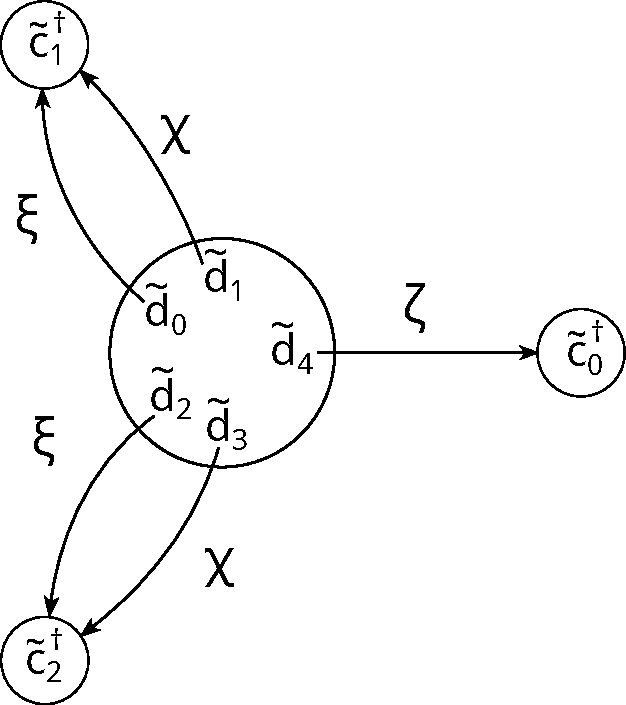
\includegraphics[width =0.95\textwidth]{Plots/3band.pdf}
\end{columns}
\end{frame}
\end{document}